\section*{Exercise Part (B) - Generate RISC Code for The Chacha20 Stream Cipher}

\begin{enumerate}[wide, label=(B\arabic*)]

% (B1) Create an excel timing-diagram for the un-optimized RISC code, of the first 3 lines of the QUARTER-ROUND operation. Use the 7-stage pipeline in part B. You may assume that a register (say R0) contains the address of the first word of the block. (Your RISC code in parts B1 to B4 should show how all memory addresses are calculated, so use explicit memory addresses in your RISC instructions, ie LOAD R1,0(R0), where the memory address is 0+R0).
% • Highlight any assumptions that you make. Use a label, ie “ASSUMPTION #1” and explain it.
\item The unoptimized RISC code for the first 3 lines of the QUARTER-ROUND operation is shown in Listing~\ref{list:b1}. The following assumptions are made for this RISC code:
\begin{itemize}
	\item ASSUMPTION 1: assume that register R0 contains the address of the first word of the block of the initial key-stream
	\item ASSUMPTION 2: each word is 32 bits, so use LD and SD instead of LW and SD to load 32-bit words
	\item ASSUMPTION 3: words in the initial key-stream are stored consecutively in memory, address of second word is address of first world + 4 (bytes)
	\item ASSUMPTION 4: assume dual-ported memory that allows simultaneous read+read, read+write, write+write
\end{itemize}
\lstinputlisting[caption=Unoptimized RISC code for the first 3 lines of QUARTER-ROUND operation,label=list:b1,firstline=6,numbers=left]{../assembly/b1.s}
The timing diagram can be seen in Figure~\ref{fig:B1}.
\begin{figure}[htp]
	\centering
	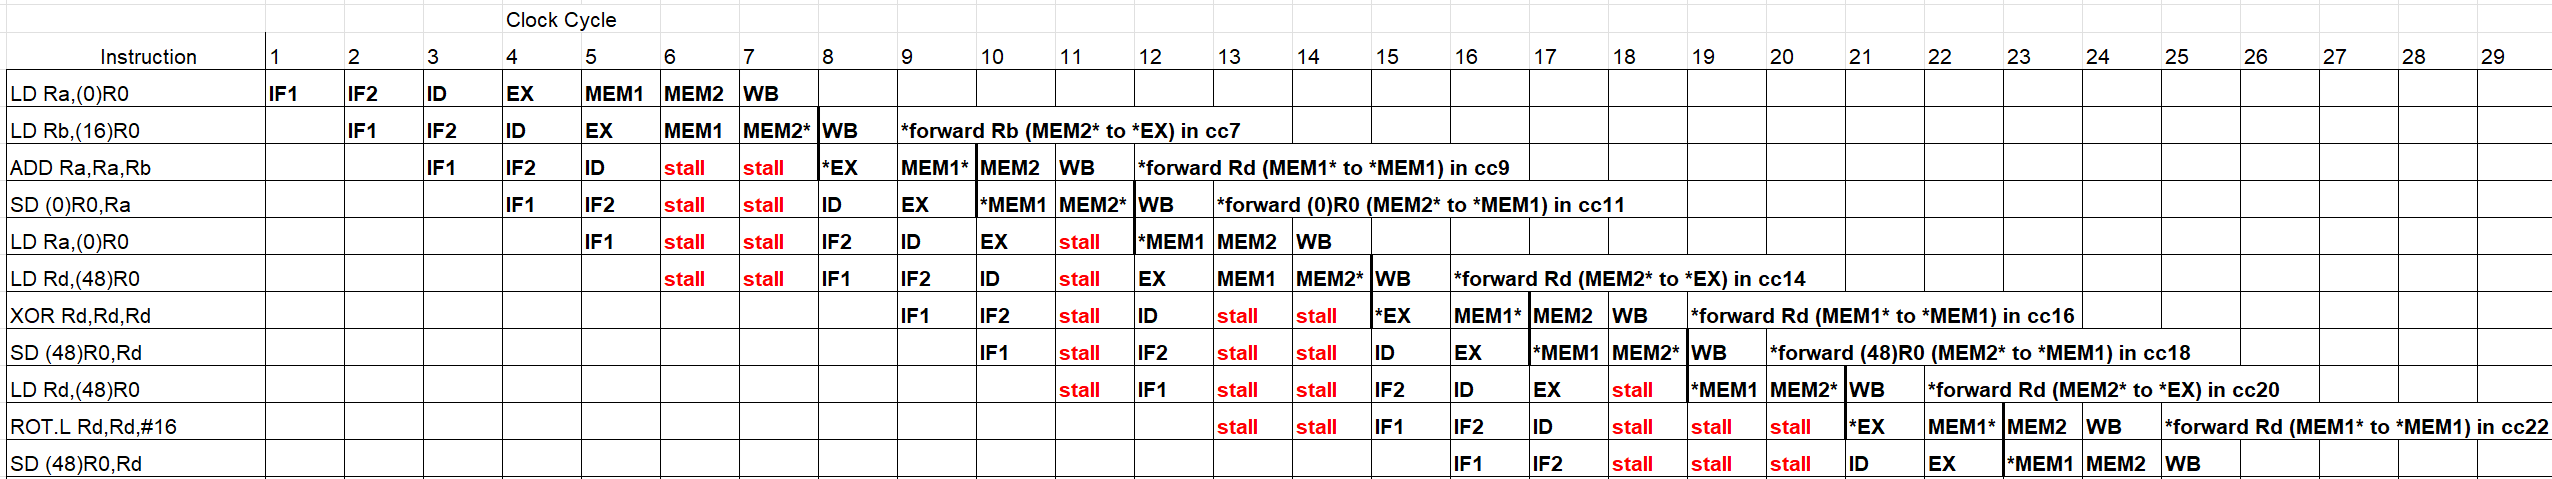
\includegraphics[width=\textwidth]{b1.png}
	\caption{\label{fig:B1}Timing Diagram for B1}
\end{figure}

% Write the un-optimized RISC code, for one QUARTER-ROUND operation (with 12 lines of C-code as shown in Fig. 2). (Use your insights gathered from B1.)
% Your answer can be a table with 3 columns: Column 1 is the RISC instruction. Column 2 is the number of stall cycles associated with that instruction. Column 3 can be a comment. You do not need to create a detailed timing-table.
% • Add a comment for every line of code. (Clear and concise comments take thought, and are worth marks.)
\item The unoptimized RISC code for one QUARTER-ROUND operation (along with the associated stall cycles per instruction) is shown in Table~\ref{tab:B2}. We make the same assumptions as we did in B1. The following macros are defined:
\lstinputlisting[caption=B2 Macros,label=list:b2,firstline=6,lastline=6]{../assembly/b2.s}
\begin{longtable}{|l|l|l|}
\caption{Unoptimized RISC code for QUARTER-ROUND operation}\label{tab:B2}\\

\hline \multicolumn{1}{|c|}{Instruction} &
\multicolumn{1}{c|}{Number of stall cycles} &
\multicolumn{1}{c|}{Comment} \\ \hline
\endfirsthead

\multicolumn{3}{c}%
{{\tablename\ \thetable{} -- continued from previous page}} \\
\hline \multicolumn{1}{|c|}{Instruction} &
\multicolumn{1}{c|}{Number of stall cycles} & 
\multicolumn{1}{c|}{Comment} \\ \hline
\endhead

\hline \multicolumn{3}{|r|}{{Continued on next page}} \\ \hline
\endfoot

\hline
\endlastfoot	

LD Ra,(0)R0	& 0	& load a from memory  \\ \hline
LD Rb,(16)R0	& 0	& load b from memory  \\ \hline
ADD Ra,Ra,Rb	& 2	& a = a + b           \\ \hline
SD (0)R0,Ra	& 2	& store a in memory   \\ \hline
LD Ra,(0)R0	& 3	& load a from memory  \\ \hline
LD Rd,(48)R0	& 3	& load d from memory  \\ \hline
XOR Rd,Rd,Ra	& 3	& XOR(d,a)            \\ \hline
SD (48)R0,Rd	& 3	& store d in memory   \\ \hline
LD Rd,(48)R0	& 4	& load d from memory  \\ \hline
ROT.L Rd,Rd,\#16	& 5	& ROTATE\_LEFT(d, 16) \\ \hline
SD (48)R0,Rd	& 3	& store d in memory   \\ \hline
LD Rc,(32)R0	& 3	& load c from memory  \\ \hline
LD Rd,(48)R0	& 3	& load d from memory  \\ \hline
ADD Rc,Rc,Rd	& 2	& c = c + d           \\ \hline
SD (32)R0,Rc	& 2	& store c in memory   \\ \hline
LD Rb,(16)R0	& 3	& load b from memory  \\ \hline
LD Rc,(32)R0	& 3	& load c from memory  \\ \hline
XOR Rb,Rb,Rc	& 3	& XOR(b,c)            \\ \hline
SD (16)R0,Rb	& 3	& store b in memory   \\ \hline
LD Rb,(16)R0	& 4	& load b from memory  \\ \hline
ROT.L Rb,Rb,\#12	& 5	& ROTATE\_LEFT(b, 12) \\ \hline
SD (16)R0,Rb	& 3	& store b in memory   \\ \hline
LD Ra,(0)R0	& 3	& load a from memory  \\ \hline
LD Rb,(16)R0	& 3	& load b from memory  \\ \hline
ADD Ra,Ra,Rb	& 2	& a = a + b           \\ \hline
SD (0)R0,Ra	& 2	& store a in memory   \\ \hline
LD Ra,(0)R0	& 3	& load a from memory  \\ \hline
LD Rd,(48)R0	& 3	& load d from memory  \\ \hline
XOR Rd,Rd,Ra	& 3	& XOR(d,a)            \\ \hline
SD (48)R0,Rd	& 3	& store d in memory   \\ \hline
LD Rd,(48)R0	& 4	& load d from memory  \\ \hline
ROT.L Rd,Rd,\#8	& 5	& ROTATE\_LEFT(d, 8)  \\ \hline
SD (48)R0,Rd	& 3	& store d in memory   \\ \hline
LD Rc,(32)R0	& 3	& load c from memory  \\ \hline
LD Rd,(48)R0	& 3	& load d from memory  \\ \hline
ADD Rc,Rc,Rd	& 2	& c = c + d           \\ \hline
SD (32)R0,Rc	& 2	& store c in memory   \\ \hline
LD Rb,(16)R0	& 3	& load b from memory  \\ \hline
LD Rc,(32)R0	& 3	& load c from memory  \\ \hline
XOR Rb,Rb,Rc	& 3	& XOR(b,c)            \\ \hline
SD (16)R0,Rb	& 3	& store b in memory   \\ \hline
LD Rb,(16)R0	& 4	& load b from memory  \\ \hline
ROT.L Rb,Rb,\#7	& 5	& ROTATE\_LEFT(b, 7)  \\ \hline
SD (16)R0,Rb	& 3	& store b in memory   \\ \hline
\end{longtable}

% (B3) Calculate the number of clock-cycles for the un-optimized QUARTER-ROUND in B2 to execute. (You can ignore the time to flush the pipeline.) Explain your answer clearly.
\item The unoptimized QUARTER-ROUND in B2 will take 82 clock-cycles to execute. We extended the the timing diagram for B1 (Figure~\ref{fig:B1}) till after the next set of LOAD instructions, and discovered that the timing diagram repeats starting on the first arithmetic operation of the next column (as seen in Figure~\ref{fig:B2}). This allowed us to extend the timing diagram to cover the entire odd ROUND operation, and we determined from the timing diagram that this operation would take 82 clock-cycles to execute.
\begin{figure}[htp]
	\centering
	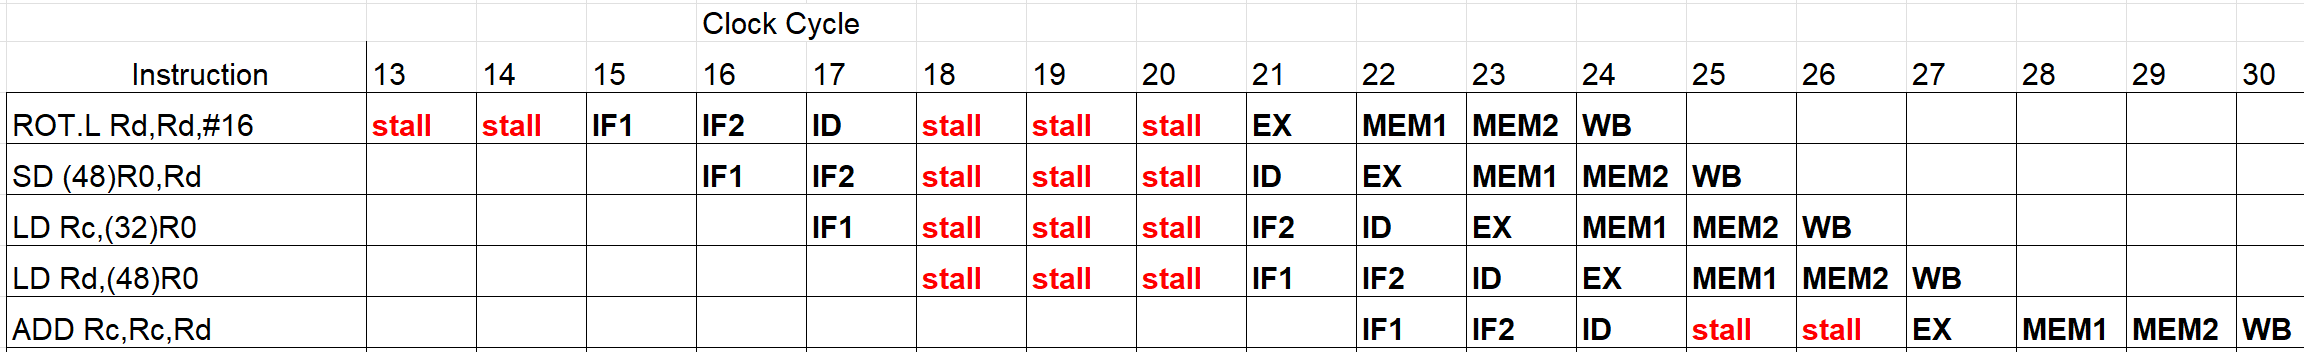
\includegraphics[width=\textwidth]{b2.png}
	\caption{\label{fig:B2}Partial Timing Diagram for B2}
\end{figure}

% (B4) Optimize the QUARTER-ROUND code in B2, to minimize stalls. (The compiler will re- arrange instructions, to minimize stalls. The compiler will minimize the number of LOADs and STORES, to minimize stalls.) Create a compressed timing-diagram, to show how the QUARTER-ROUND will execute once it has been optimized. The timing-diagram will illustrate how many stalls occur. Explain how many clock cycles it takes, to execute the optimized QUARTER-ROUND operation.
% In the compressed timing diagram, use comments to indicate all forwarding of data and signals. A comment might be ‘* forward R0 (EX to D) in cc 7’. (If you have already made an uncompressed timing diagram, you can use that instead.)
\item When we optimize the QUARTER-ROUND code in B2, we are able to reduce the number of clock cycles required to execute the QUARTER-ROUND operation from 82 clock-cycles to just 26. The compressed timing diagram and the optimized QUARTER-ROUND code can be seen in Table~\ref{tab:B4}. We make the same assumptions as we did in B1. The following macros are defined:
\lstinputlisting[caption=B4 Macros,label=list:b4,firstline=6,lastline=6]{../assembly/b4.s}

% (B5) Generate the optimized RISC code for one ROUND which operates on the 4 COLUMNs of a block. One simple solution here is to repeat your optimized code from B4 for each column of the block, (ie repeat 4 times for 4 columns). (However, this code might not be optimized. You should optimize it, if possible.) Create a table with 3 columns, to show how one ROUND will execute once it has been optimized. Column 1 identifies a block of RISC code (it might be a QR from B4, or a subset of a QR from B4.) Column 2 illustrates the number of clock cycles, and stall cycles, associated with that block of RISC code. Column 3 can be a comment, as shown below. (Show the memory addresses of the variables A,B,C,D that you use, for each column.) If you move any code around to optimize it, explain which code from which QR is moved, and explain where it is moved to.
% Explain how many clock cycles it takes, to execute the optimized ROUND operation. (You can ignore the time to flush the pipeline.) Explain your answer clearly; a numerical answer alone may not be sufficient.
\item The optimized RISC code for one ROUND which operates on the 4 COLUMNs of a block is simply the optimized QUARTER-ROUND operation from B4 repeated four times, but with different memory addresses used for each QUARTER-ROUND operation. The code for the ROUND operation is described in Table~\ref{tab:B5}. We do not need to modify the code for the QUARTER-ROUND operation as there is no stalling between the columns even if the code is repeated as-is. We make the same assumptions as we did in B1. In each iteration of the QUARTER-ROUND operation, the only changes are the memory addresses used for loading registers Ra, Rb, Rc, and Rd at the start of the QUARTER-ROUND operation. The following macros are defined:
\lstinputlisting[caption=B5 Macros,label=list:b5,firstline=6,lastline=6]{../assembly/b5.s}

From the table, we can see that it would simply take 4 $\times$ the number of clock-cycles per QUARTER-ROUND operation or $4 \times 26 = 104$ clock-cycles.

\begin{table}[htp]
\centering
\resizebox{\textwidth}{!}{
\begin{tabular}{|l|c|c|c|c|c|l|}
		\hline
		Instruction        & F1,F2 & D 	& EX       & M1,M2   & WB & \multicolumn{1}{c|}{Comments}        \\ \hline
		LD Ra,(0)R0        & 1,2   & 3 	& 4        & 5,6     & 7  &                                      \\ \hline
		LD Rb,(16)R0       & 2,3   & 4 	& 5        & 6,7*    & 8  & * forward Rb (M2 to EX) end of cc7   \\ \hline
		LD Rd,(48)R0       & 3,4   & 5 	& 6        & 7,8*    & 9  & * forward Rd (M2 to EX) end of cc8   \\ \hline
		LD Rc,(36)R0       & 4,5   & 6 	& 7        & 8,9     & 10 &                                      \\ \hline
		ADD Ra,Ra,Rb       & 5,6   & 7 	& *8**     & 9,10    & 11 & ** forward Ra (EX to EX) end of cc8  \\ \hline
		XOR Rd,Rd,Ra       & 6,7   & 8 	& *,**9*** & 10,11   & 12 & *** forward Rd (EX to EX) end of cc9 \\ \hline
		ROT.L   Rd,Rd,\#16 & 7,8   & 9 	& ***10*   & 11,12   & 13 & * forward Rd (EX to EX) end of cc10  \\ \hline
		ADD Rc,Rc,Rd       & 8,9   & 10	& *11**    & 12,13   & 14 & ** forward Rc (EX to EX) end of cc11 \\ \hline
		XOR Rb,Rb,Rc       & 9,10  & 11	& **12*    & 13,14   & 15 & * forward Rb (EX to EX) end of cc12  \\ \hline
		ROT.L   Rb,Rb,\#12 & 10,11 & 12	& *13**    & 14,15   & 16 & ** forward Rb (EX to EX) end of cc13 \\ \hline
		ADD Ra,Ra,Rb       & 11,12 & 13	& **14*    & 15,16   & 17 & * forward Ra (EX to EX) end of cc14  \\ \hline
		XOR Rd,Rd,Ra       & 12,13 & 14	& *15**    & 16,17   & 18 & ** forward Rd (EX to EX) end of cc15 \\ \hline
		ROT.L Rd,Rd,\#8    & 13,14 & 15	& **16*    & 17,18   & 19 & * forward Rd (EX to EX) end of cc16  \\ \hline
		ADD Rc,Rc,Rd       & 15,16 & 16	& *17**    & 18,19   & 20 & ** forward Rc (EX to EX) end of cc17 \\ \hline
		XOR Rb,Rb,Rc       & 17,18 & 17	& **18*    & 19,20   & 21 & * forward Rb (EX to EX) end of cc18  \\ \hline
		ROT.L Rb,Rb,\#7    & 18,19 & 18	& *19      & 20,21** & 22 & ** forward Rb (M2 to ID) end of cc21 \\ \hline
		SD (0)R0,Ra        & 19,20 & 19	& 20       & 21,22   & 23 &                                      \\ \hline
		SD (48)R0,Rd       & 20,21 & 20	& 21       & 22,23   & 24 &                                      \\ \hline
		SD (32)R0,Rc       & 21,22 & 21	& 22       & 23,24   & 25 &                                      \\ \hline
		SD (16)R0,Rb       & 22,23 & **22	& 23       & 24,25   & 26 &                                      \\ \hline
		\end{tabular}
	}
\caption{Optimized QUARTER-ROUND operation}\label{tab:B4}
\end{table}

\begin{table}[htp]
\centering
\resizebox{\textwidth}{!}{
\begin{tabular}{|l|l|l|}
	\hline
	Code &
		Clock Cycles &
		Comment \\ \hline
	B4 QR((0)R0,(16)R0,(32)R0,(48)R0 &
		\begin{tabular}[c]{@{}l@{}}26 clock cycles to execute\\ 0 clock cycles for stalls\end{tabular} &
		\begin{tabular}[c]{@{}l@{}}(0)R0, (16)R0, (32)R0, (48)R0 are the addresses\\ for words 0, 4, 8, 12 (first column)\end{tabular} \\ \hline
	B4 QR((4)R0,(20)R0,(36)R0,(52)R0) &
		\begin{tabular}[c]{@{}l@{}}26 clock cycles to execute\\ 0 clock cycles for stalls\end{tabular} &
		\begin{tabular}[c]{@{}l@{}}(4)R0, (20)R0, (36)R0, (52)R0 are the addresses\\ for words 1, 5, 9, 13 (second column)\end{tabular} \\ \hline
	B4 QR((8)R0,(24)R0,(40)R0,(56)R0) &
		\begin{tabular}[c]{@{}l@{}}26 clock cycles to execute\\ 0 clock cycles for stalls\end{tabular} &
		\begin{tabular}[c]{@{}l@{}}(8)R0, (24)R0, (40)R0, (56)R0 are the addresses\\ for words 2, 6, 10, 14 (third column)\end{tabular} \\ \hline
	B4 QR((12)R0,(28)R0,(44)R0,(60)R0) &
		\begin{tabular}[c]{@{}l@{}}26 clock cycles to execute\\ 0 clock cycles for stalls\end{tabular} &
		\begin{tabular}[c]{@{}l@{}}(12)R0, (28)R0, (44)R0, (60)R0 are the addresses\\ for words 3, 7, 11, 15 (fourth column)\end{tabular} \\ \hline
\end{tabular}
}
\caption{ROUND operation}\label{tab:B5}
\end{table}

%(B6) Generate the optimized RISC code for the outer loop and inner loop of Chacha20. The outer loop will process B blocks of key-stream. The inner-loop will have 10 iterations, of the DOUBLE-ROUND operation in Fig 3. (You do not need to write out all the RISC code for the double-round, as you can verbally explain that you use the code from B5 for each round in the inner loop.)
% Explain any of your optimizations: If you move any code around for optimization, please explain which lines of code were moved, explain where they were moved from, and where they were moved to.
% Your answer can be a table with 3 columns: Column 1 can refer to a RISC instruction (or block of RISC code). Column 2 is the number of stall cycles associated with that instruction or block of RISC code. Column 3 can be a comment. You do not need to create a detailed timing-table. (In the 1st column, a RISC instruction could also say: “Insert RISC code from B5 for one round’. The number of stalls for that code can go into the 2nd column.)
% • Add a comment for every line of code. (Clear and concise comments take thought, and are worth marks.)
% Clearly explain how many clock cycles it takes, to process 1,024 blocks of data. Explain how many clock cycles it takes, to execute the optimized outer and inner loops for Chacha20. If any instructions cause stalls, identify these instructions, and explain how many stalls per instruction occur. (You can ignore the time to flush the pipeline.)
% • If you make any assumptions, highlight those assumptions. Use a label ie “ASSUMPTION #1” and explain it.
\item The optimized RISC code and the outer and inner loop of Chacha20 can be seen in Table~\ref{tab:B6}. For the DOUBLE-ROUND operation in the inner loop, the first ROUND operation uses the unmodified code from B5, while the second ROUND operation updates the addresses for the diagonals. We also exclude the last STORE instruction from our diagonal ROUND operation, so we can place it after the BNEZ instruction to use one of our branch-delay-slots (there are 2 branch-delay-slots after each branch as shown in A2). We also fill our remaining branch-delay-slots with useful instructions which allows to have a Chacha20 operation with no stalling. The following assumptions are made for this RISC code:
\begin{itemize}
	\item ASSUMPTION 1: assume that register R0 contains the address of the first word of the block of the initial key-stream
	\item ASSUMPTION 2: each word is 32 bits, so use LD and SD instead of LW and SD to load 32-bit words
	\item ASSUMPTION 3: words in the initial key-stream are stored consecutively in memory, address of second word is address of first world + 4 (bytes)
	\item ASSUMPTION 4: assume dual-ported memory that allows simultaneous read+read, read+write, write+write
\end{itemize}
The following macros are defined:
\lstinputlisting[caption=B6 Macros,label=list:b6,firstline=6,lastline=7]{../assembly/b6.s}

\begin{table}[htp]
\centering
\caption{Outer and Inner Loops of Chacha20}\label{tab:B6}
\resizebox{\textwidth}{!}{
\begin{tabular}{|l|l|l|}
	\hline
	Code &
		Number of stall cycles &
		Comment \\ \hline
	LW.I    Rlo,\#1023 &
		0 &
		initialize loop counter for outer loop for 1024 blocks \\ \hline
	outer\_loop:    LW.I    Rli,\#9 &
		0 &
		\begin{tabular}[c]{@{}l@{}}start of outer loop\\ initialize loop counter for inner loop for 10 iterations\\ of DOUBLE-ROUND\end{tabular} \\ \hline
	\begin{tabular}[c]{@{}l@{}}inner\_loop:\\ Insert RISC code from B5 for one round\end{tabular} &
		0 &
		\begin{tabular}[c]{@{}l@{}}start of inner loop\\ odd round\\ unmodified code from B5\end{tabular} \\ \hline
	\begin{tabular}[c]{@{}l@{}}Insert RISC code from B5 for one round\\ with modified diagonal addressing\\ excluding SD instruction\end{tabular} &
		0 &
		\begin{tabular}[c]{@{}l@{}}even round\\ update B5 code to have addressing for diagonals\\ (QR((0)R0,(20)R0,(40)R0,(60)R0), ...)\\ exclude last store instruction to place in\\ branch-delay-slot\end{tabular} \\ \hline
	BNEZ    Rli,inner\_loop &
		0 &
		repeat inner\_loop if inner loop counter not 0 \\ \hline
	SD    (x)R0,Rb &
		0 &
		\begin{tabular}[c]{@{}l@{}}use branch-delay-slot\\ last store instruction from even ROUND\end{tabular} \\ \hline
	SUB.I    Rli,\#1 &
		0 &
		\begin{tabular}[c]{@{}l@{}}use branch-delay-slot\\ decrement inner loop counter by 1\end{tabular} \\ \hline
	BNEZ   Rlo,outer\_loop &
		0 &
		repeat outer loop if outer loop counter not 0 \\ \hline
	ADD.I    R0,\#64 &
		0 &
		\begin{tabular}[c]{@{}l@{}}use branch-delay-slot\\ increment address to next block (4 * 16 bytes)\end{tabular} \\ \hline
	SUB.I    Rlo,\#1 &
		0 &
		\begin{tabular}[c]{@{}l@{}}use branch-delay-slot\\ decrement outer loop counter by 1\end{tabular} \\ \hline
\end{tabular}
}
\end{table}

% Assume a 2.5 GHz clock rate. Assume a RISC machine that fetches 1 instruction at a time. How long does it take (in nanoseconds, microseconds, or milliseconds) to process 1,024 blocks, in part B5 ? Explain your answer clearly; a numerical answer alone may not be sufficient.
\item For the optimized RISC code for a QUARTER-ROUND operation in B4, we had 20 instructions. Therefore, each ROUND operation contains 80 instructions. The inner loop in B6 contains 162 instructions (80 from first ROUND, 79 from second ROUND, 1 from branch, 2 from branch-delay-slots), and this iterates 10 times in every iteration of the outer loop for 1620 instructions. Each outer loop iteration contains 1624 instructions (1 from inner loop counter initialization, 1620 from inner loop, 1 from branch, 2 from branch-delay-slots), iterated 1024 times for a total of 1662976 instructions. Once we add the instruction for the outer loop counter initialization, and the 6 extra instructions for the last Chacha20 instruction to finish the WB stage of the pipeline, we are left with 1662983 instructions.

With a 2.5 GHz clock rate, we can process 2500000000 instructions per second. This means we can process 1662983 instructions in 0.665193 milliseconds, or 665.1932 microseconds.

\end{enumerate}